\subsection{Zadanie 2.3 Minimalizacja terminu realizacji puli projektów}
\begin{figure}[htb]
\caption{Czas realizacji projektów}
\begin{center}
\begin{tabular}{ | c | c | c | c | c | c | c | }
\hline
  & A & B & C & D & E & F \\ 
 \hline
 1 & - & 13 & - & 14 & 18 & - \\  
 \hline
 2 & - & 4 & 2 & - & 3 & - \\
 \hline  
 3 & 2 & - & - & 10 & - & 13 \\
 \hline  
 4 & 10 & - & 5 & - & - & 15 \\
 \hline  
 5 & - & 10 & - & - & 17 & 12 \\
 \hline  
 6 & 20 & - & 6 & 16 & - & - \\
 \hline
\end{tabular}
\end{center}
\end{figure}

\begin{enumerate}
\item Parametry \\
s - źródło \\
w - wyjście \\
N - węzły (N = {s, t, 1, 2, 3, 4, 5, 6, A, B, C, D, E, F})
P - projekty (P = {1, 2, 3, 4, 5, 6} $\subseteq$ N)
Z - zespoły (Z = {A, B, C, D, E, F} $\subseteq$ N)
$t_{zp}$  - czas realizacji projektu p przez zespół z [w miesiącach]

\item Zmienne decyzyjne:
$f_{ij}$ - przeływ pomiędzy węzłem i oraz węzłem j
\item Funkcja celu
\begin{align*}
    Q &= \min \left( \max_{z \in Z, p \in P} c_{zp} f_{zp} \right) \\
    &= \min \big\{13f_{B1}, 14f_{D1}, 18f_{E1}, 4f_{B2}, 2f_{C2}, 3f_{E2}, \\
    &\quad  2f_{A3}, 10f_{D3},13f_{F3}, 10f_{A4}, 5f_{C4}, 15f_{F4} \\
    &\quad 10f_{B5}, 17f_{E5}, 12f_{F5}, 20f_{A6}, 6f_{C6}, 16f_{D6} \big\}
\end{align*}


\item Ograniczenia
\setcounter{equation}{0}
\begin{equation}
0 \leq f_{ij} \leq 1, \; (i, j) \in N
\end{equation}
\begin{equation}
f_{si} = 0, \; i \in \{ s, t, 1, 2, 3, 4, 5, 6 \}
\end{equation}
\begin{equation}
f_{is} = 0, \; i \in N
\end{equation}
\begin{equation}
f_{ti} = 0, \; i \in N
\end{equation}
\begin{equation}
f_{it} = 0, \; i \in \{s, t, A, B, C, D, E, F\}
\end{equation}
\begin{equation}
\sum_{z \in Z} f_{zp} = 1, \; p \in P = \{ 1, 2, 3, 4, 5, 6 \}
\end{equation} 
\begin{equation}
\sum_{p \in P} f_{zp} = 1, \; z \in Z = \{ A, B, C, D, E, F \}
\end{equation}
\begin{equation}
\sum_{i \in N \backslash \{s\}} f_{ni} = \sum_{j \in N \backslash \{t\}} f_{jn}, \; n \in N \backslash \{ s, t \}
\end{equation}

\end{enumerate}
\paragraph{Model sieciowy rysunek}
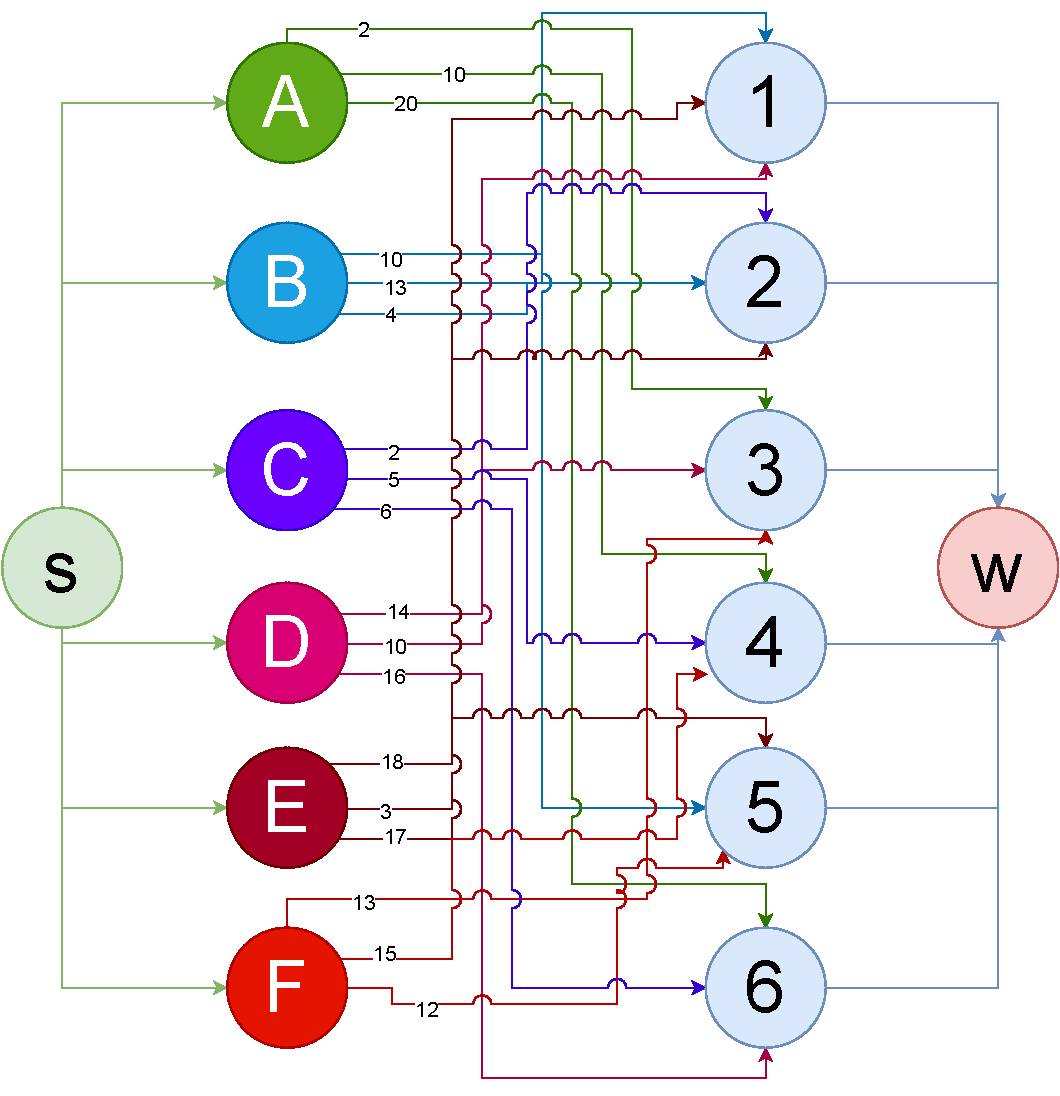
\includepdf[pages=-]{flowchart22.pdf}
\paragraph{Model programowania liniowego}
\begin{lstlisting}[caption= plik dat]
data; 
 
set Wyjscie := t; 
set Wezly := 1, 2, 3, 4, 5, 6, A, B, C, D, E, F; 
set StartWezly := s, 1, 2, 3, 4, 5, 6, A, B, C, D, E, F; 
set WyjscieWezly := t, 1, 2, 3, 4, 5, 6, A, B, C, D, E, F; 
set StartWyjscieWezly := s, t, 1, 2, 3, 4, 5, 6, A, B, C, D, E, F; 
set Projekty := 1, 2, 3, 4, 5, 6; 
set Zespoly := A, B, C, D, E, F; 
 
param c := 
A 1 1000 A 2 1000 A 3 2 A 4 10 A 5 1000 A 6 20
B 1 13 B 2 4 B 3 1000 B 4 1000 B 5 10 B 6 1000 
C 1 1000 C 2 2 C 3 1000 C 4 5 C 5 1000 C 6 6 
D 1 14 D 2 1000 D 3 10 D 4 1000 D 5 1000 D 6 16 
E 1 18 E 2 3 E 3 1000 E 4 1000 E 5 17 E 6 1000 
F 1 1000 F 2 1000 F 3 13 F 4 15 F 5 12 F 6 1000; 
 
end; 
\end{lstlisting}
\begin{lstlisting}[caption= plik mod]
set Wyjscie; 
set Wezly; 
set StartWezly; 
set WyjscieWezly; 
set StartWyjscieWezly; 
set Projekty; 
set Zespoly; 
 
param c{z in Zespoly, p in Projekty}; 
 
var f{i in StartWyjscieWezly, j in StartWyjscieWezly}, >= 0, integer; 
var cmax, >= 0; 
 
minimize Q: cmax; 
 
subject to
  Ograniczenie_jeden{i in StartWyjscieWezly, j in StartWyjscieWezly}: 
    f[i,j] >= 0; 
  Ograniczenie_dwa{i in StartWyjscieWezly, j in StartWyjscieWezly}: 
    f[i,j] <= 1; 
  Ograniczenie_trzy{p in Projekty}: 
    sum {z in Zespoly} f[z,p] = 1; 
  Ograniczenie_cztery{z in Zespoly}: 
    sum {p in Projekty} f[z,p] = 1; 
  Ograniczenie_piec{n in Wezly}: 
    sum {i in WyjscieWezly} f[n,i] = sum {j in StartWezly} f[j,n]; 
	Ograniczenie_szesc{z in Zespoly, p in Projekty}: 
		c[z,p] * f[z,p] <= cmax;
solve;
display {i in Wezly, j in Wezly: f[i,j] > 0}: f[i,j]; 
display: Q;
\end{lstlisting}

\begin{lstlisting}[caption=wynik z glpk]
f[A,4].val = 1
f[B,1].val = 1
f[C,6].val = 1
f[D,3].val = 1
f[E,2].val = 1
f[F,5].val = 1
Q.val = 13
\end{lstlisting}
Wyniki: \\
Projekt numer \textbf{1} zostanie przydzielony zespołowi \textbf{B} \\
Projekt numer \textbf{2} zostanie przydzielony zespołowi \textbf{E} \\
Projekt numer \textbf{3} zostanie przydzielony zespołowi \textbf{D} \\
Projekt numer \textbf{4} zostanie przydzielony zespołowi \textbf{A} \\
Projekt numer \textbf{5} zostanie przydzielony zespołowi \textbf{F} \\
Projekt numer \textbf{6} zostanie przydzielony zespołowi \textbf{C} \\
